
\section{Structural Frame } \label{sec:struc} 
The structural frame has its history in the frame defined by the
manufacturer of a vehicle for fabrication reference and vehicle body reference operations. It is often defined with the X-axis directed aft, the Y-axis directed toward the right, and the Z-axis directed upward. On some vehicles the centerline serves as the X-axis, with the origin of the coordinate system either at the tip of the vehicle nose, or somewhere out in front of it. Iin the case of the space shuttle, the X-axis was parallel to the longitudinal axis of the payload bay with positive toward the tail, and frame was centered 400 inches below the centerline of the payload bay. A candidate body is picked to demonstrate a structural body axes system.

\textbf{Coordinate Frame:} Non Inertial.

\begin{itemize}
\item X-axis: The X-axis coincides with the centerline of the cone and is positive from the cone apex toward a heat-shield. This orientation , in this example,  is dictated by the use of heritage Shuttle hardware as components.
\item Y-axis:Completes the right-handed system, resulting in the positive direction toward the crew's right when the crew is seated facing the cone apex.
\item Z-axis:The Z-axis lies in the plane containing the origin and a line equidistant between the 2 windows. The positive Z direction corresponds to the "feet to head" direction for the seated crew.
\textbf{The following figure is only an example a user or project is free to choose a convenient structural body axis system.}
\end{itemize}


\begin{figure}[htp]
\centering
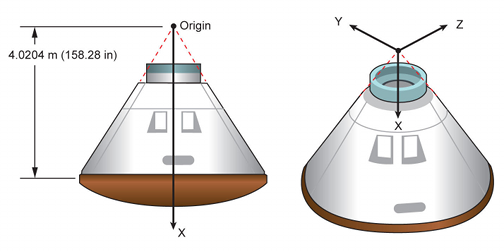
\includegraphics [width=7in]{figs/fig11.png}
\caption{Structural System}
\label{fig:11}
\end{figure}

\subsection{Example Sructural Frame}
For a simple example see:
\begin{verbatim}
jeod\verif\SIM_dyncomp\SET_test\RUN_10A
\end{verbatim}


